\documentclass[conference]{IEEEtran}

\usepackage[noadjust]{cite}
\usepackage{amsmath}
\usepackage{amsfonts}
\usepackage{amssymb}
\usepackage{graphicx}
\usepackage[utf8]{inputenc}
\usepackage{pdfpages}

\title{Using part of speech in tweet classification\\
\normalsize Kaggle group name: POS-itive}
\author{\IEEEauthorblockN{Richard Wigren}
		\IEEEauthorblockN{17-909-383} 
		\and 
		\IEEEauthorblockN{Michiel Baptist}
		\IEEEauthorblockN{17-907-544} 
		\and 
		\IEEEauthorblockN{Gorm Rødder}
		\IEEEauthorblockN{17-908-963}}
        
\newcommand{\Glove}{GloVe }
\begin{document}
	\maketitle
	
\begin{abstract}
 Sentiment analasys is an important field, which has gained in popularity. As social media becomes more and more an important factor in marketing, so does sentiment analasys. In this paper we present a sentiment analasys technique which improves on a classical model by using part of speech information. 
\end{abstract}
	
\section{Introduction} The task of sentiment analysis consists of extracting subjective information, such as opinions and attitudes, from language \cite{Liu10sentimentanalysis}. It has been explored extensively in previous works \cite{Liu10sentimentanalysis,SA_RECENT}. In this paper we present a supervised method for classification of short pieces of text in the form of tweets into either positive or negative sentiment. In section \ref{sec:models} we present our method in an incremental fashion and present three baseline methods against which we compare our model. In section \ref{sec:results} we present results from experiments we performed on the models described in section \ref{sec:models}. Finally in section \ref{sec:discussion} we discuss the results of the experiments.
	
\section{Models and Methods}
\label{sec:models}
In this section, after some definitions, we present three baseline methods, our vanilla model, and several improvements attempted incrementally. Note that our baselines are not taken from the programming exercises.\\\\
\textbf{Tweet tokenization}: In the following models we assume a tweet consists of a string. Before classification we usually have to tokenize the tweet. We consider a tokenization as a deterministic mapping:
	\begin{equation}
	t:\mathbb{S}_{140} \rightarrow \mathbb{T}^{l(i)}
	\end{equation} Where $\mathbb{S}_{140}$ is the set of all possible strings of size less than 140 characters, $\mathbb{T}$ is the vocabulary with $|\mathbb{T}|=M$. $l(i)$ is an integer depending on the string being mapped. For notational purposes we write $t(x) = w_1,\dots,w_n$ Not all models presented use the same tokenization function. A simple example of a tokenizer is the space tokenizer which splits a string at the spaces.\\\\
\textbf{Word embedding:}
Word embeddings form a core concept in modern natural language understanding. Many models have been proposed in an attempt to capture semantic meaning of a word as a continuous vector \cite{Survey, Word2vec, GLOVE}. We consider a word embedding as a deterministic mapping:
	\begin{equation}
	e:\mathbb{T} \rightarrow \mathbb{R}^l
	\end{equation} where $\mathbb{T}$ is the vocabulary, $l$ is the length of the real vector or the embedding size.
	
\subsection{Baseline: Naive Bayes}
The Naive Bayes classifier is well known and has been successfully applied in the past, such as spam filtering and text classification \cite{NB_SPAM, NB_SAL}. The main idea of the naive Bayes classifier is that tweets with a positive sentiment might have a very different distribution over words than tweets with a negative sentiment. Concretely we consider the model:	
	\begin{equation}
		P(c|w_1, \dots, w_n) = \frac{P(c)P(w_1, \dots, w_n|c)}{P(w_1,\dots,w_n)}
	\end{equation}
	Where $w_1, \dots, w_n$ are the tokens of a tweet and $c$ is the class to which the tweet belongs. In this case either positive or negative. Making the naive Bayes assumption we assume the tokens $w_i$ are independent given the class to which it belongs, i.e.:
	\begin{equation}
	p(w_1, \dots, w_n|c) = \prod_{i=1}^{n}P(w_i|c)
	\end{equation}
	Assuming $W|c$ is a categorical random variable, we estimate $P(W=w_i|c=j) = \theta_{ij}$ using maximum likelihood with $\alpha$-smoothing as in \cite{NB_SAL}, i.e. we use the following estimates:
	\begin{equation}
		P(W=w_i|c=j) = \hat{\theta}_{ij} = \frac{N_{ij} + \alpha}{\sum_{i=1}^{M}(N_{ij} + \alpha) }
	\end{equation}
	Where $M$ is size of the vocabulary. The Bayes optimal classifier then becomes:
    \begin{equation}
    	\hat{c} = \underset{c}{\text{arg max }} P(c|w_1, \dots, w_n)
    \end{equation}
    The naive Bayes classifier was implemented using the MultinomialNaiveBayes implementation of scikit-learn \cite{sklearn}. Our $\alpha$ value is set to 1.
	
\subsection{Baseline: Averaged word embedding SVM} In order to leverage the semantic meaning captured by word embeddings we propose the following classifier as a baseline:
		\begin{enumerate}
			\item Tokenize the tweet: $t(x) = w_1, \dots, w_n$
			\item Embed the tokens: $e(w_i) = v_i \hspace{0.5 cm} \forall i \leq n$
			\item Average the word embeddings: $a = \frac{1}{n}\sum_{i=1}^{n}v_i$
			\item Classify the tweet: $\hat{c} = c(a)$
		\end{enumerate}
		Where $c$ is a classifier. We use Stanford's \Glove embeddings trained on Twitter data \cite{GLOVE} of size 200 and the implementation of Random Forests from scikit-learn \cite{sklearn} as the classifier. Note this baseline has been suggested on the tutorial slides\footnote{https://github.com/dalab/lecture\_cil\_public/blob/master\\/exercises/ex6/tutorial06.pdf}.
\subsection{Baseline: Google sentence embeddings}
In a similar vein as the previous baseline we attempt to capture semantic meaning using vectors of real numbers. However, we attempt to do this for the tweet entirely by using Google's Universal Sentence Encoder embeddings \cite{GOOGLE_SENTENCE} and classifying the semantic meaning in the form of a continuous vector as either positive or negative.\\
\indent The Google sentence embedding is a deterministic mapping $\mathbb{S} \rightarrow \mathbb{R}^{512}$, we then train a feed forward neural network classifier.
	\begin{figure}[h!]
    	\centering
		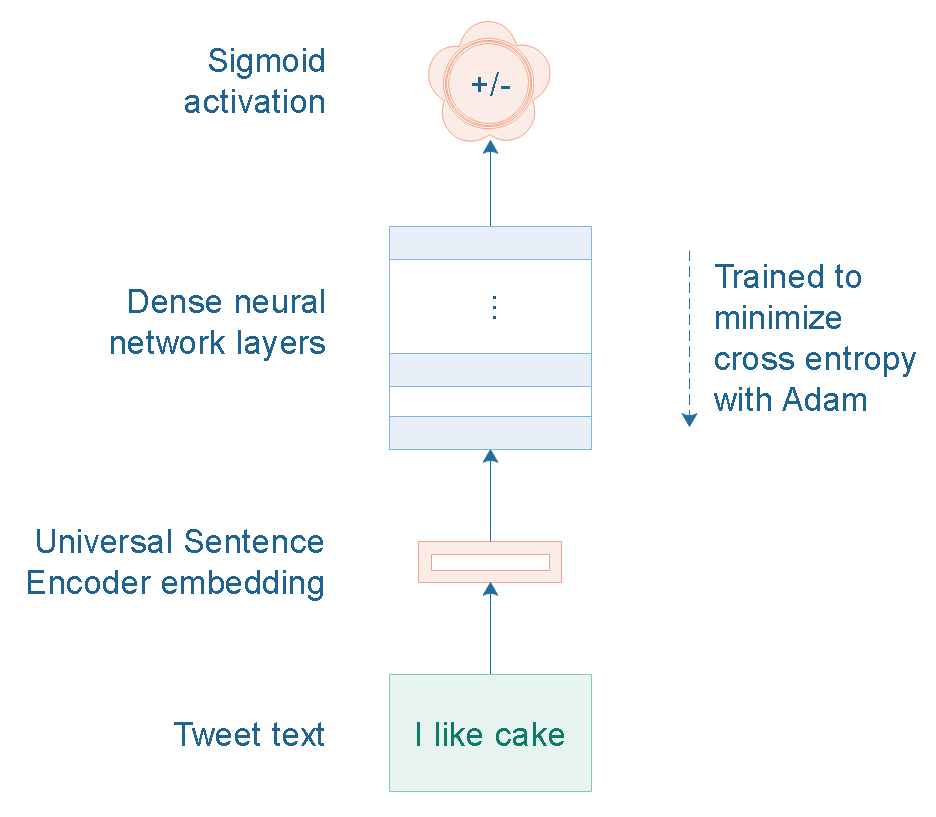
\includegraphics[scale=0.55]{fig/sentence_embedding.PNG}
        \caption{The general structure of the sentence embedding baseline. Image created using Edraw Max\cite{Edraw}.}
        \label{fig:sentence_embedding}
	\end{figure}
	Figure \ref{fig:sentence_embedding} shows the general architecture of this baseline. We attempted two different feed-forward architectures to classify the sentence embeddings:
\begin{enumerate}
	\item 4 hidden layers of size 256, 256, 128 and 64. Each hidden layer has sigmoid activations. Output of size 1 with sigmoid activation.
	\item 5 hidden layers of size 256, 256, 128, 128 and 128. Each hidden layer has sigmoid activations. Output of size 1 with sigmoid activation.
\end{enumerate} 
We use Tensorflow \cite{tensorflow} to implement the different feed forward architectures. As mentioned previously we use Google's sentence embedding \cite{GOOGLE_SENTENCE} to embed the tweets, their code has been made publically available on Tensorflow Hub\footnote{https://tfhub.dev/google/universal-sentence-encoder/2}. We use Tensorflow's Adam optimizer to minimize for cross entropy. Section \ref{sec:results} shows results for different feed-forward architectures.
		
\subsection{Model and Improvements}
LSTM recurrent neural networks \cite{LSTM, LSTM_PLUS} have been successfully applied in many areas when dealing with sequential data. Examples of good performance of LSTM networks can be found in machine translation \cite{Machine_translation}, language modeling \cite{language_modeling} and question answering \cite{question_answering}. In an attempt to leverage the predictive power of LSTM networks we propose to use a simple LSTM network as our vanilla model.
\begin{table}[h!]
\centering
\begin{tabular}{l|c}
Parameter & Value \\
\hline
Embedding & May vary\\
Cell layers & 1 \\
Cell Hidden size & 128 \\
Dense layers after output & 2 \\
Dense layer sizes & 128, 128 \\
Dense layer activations & Sigmoid, Sigmoid\\
Output layer size & 1\\
Output activation & Sigmoid\\
Objective & (binary) cross entropy\\
\end{tabular}
\caption{Overview of the parameters of the vanilla LSTM model.}
\label{tab:vanilla_params}
\end{table}
    \begin{figure}
    \centering
    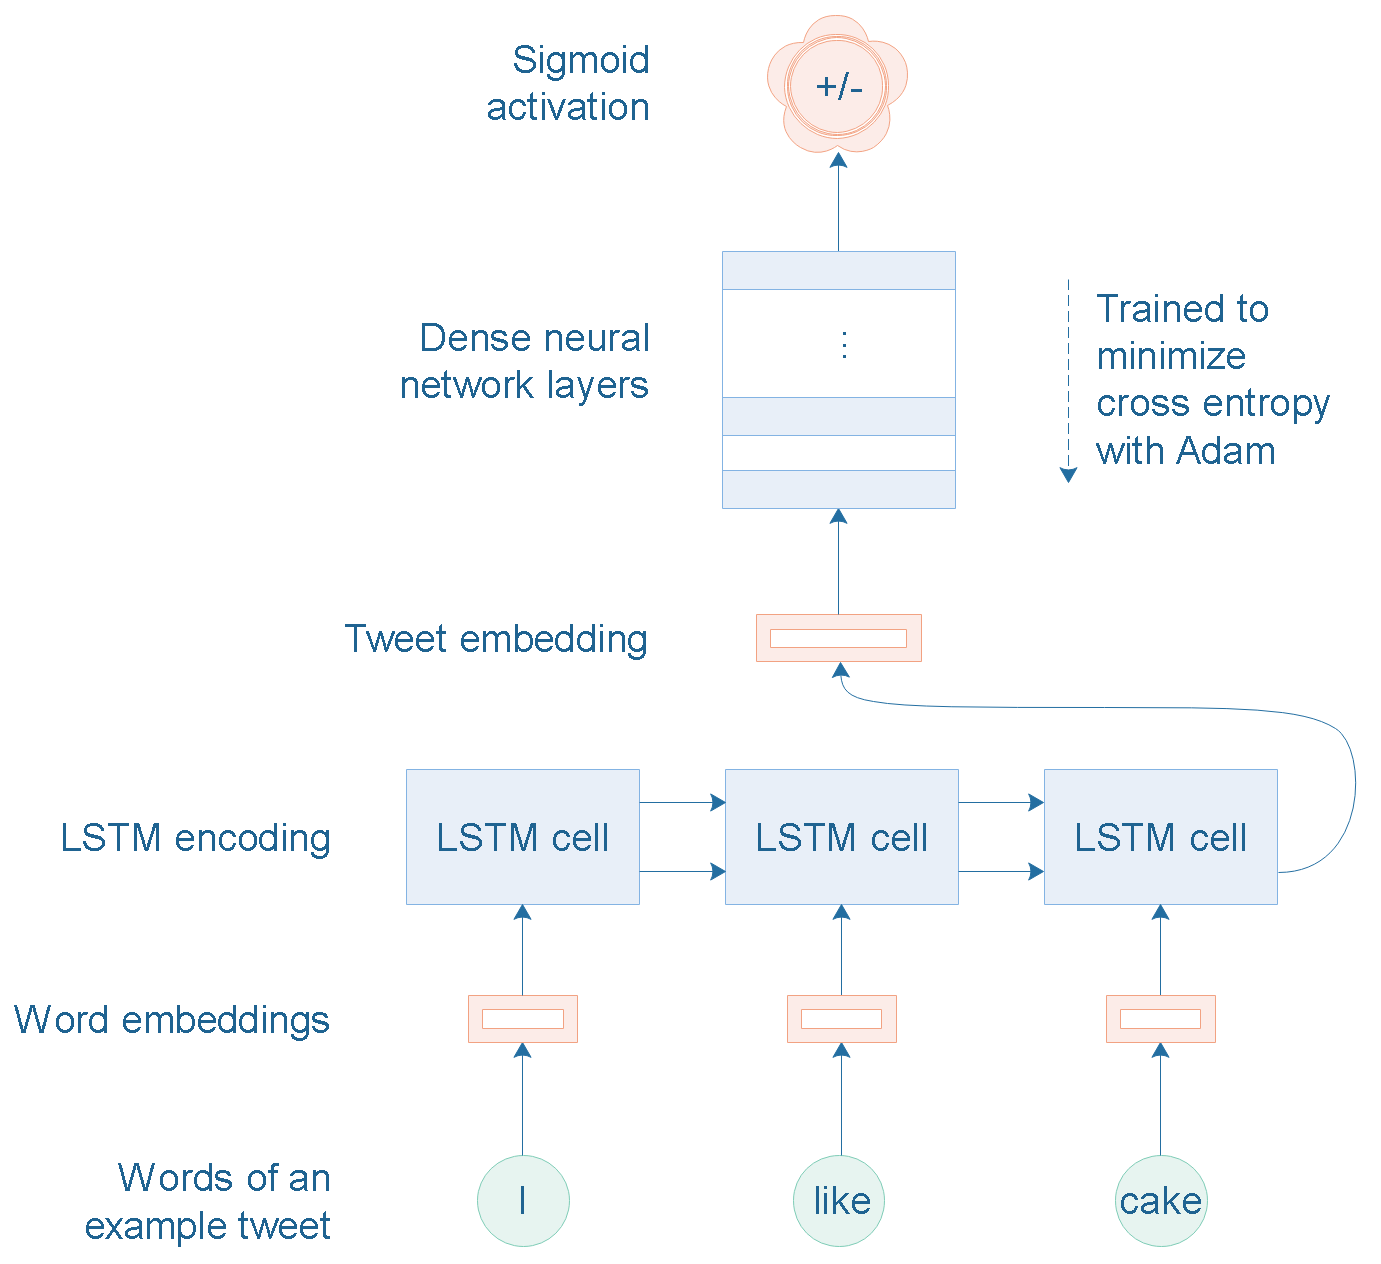
\includegraphics[scale=0.5]{fig/LSTM.PNG}
    \caption{The vanilla LSTM model architecture. Image created using Edraw Max\cite{Edraw}.}
    \label{fig:vanilla}
    \end{figure}\\
    Figure \ref{fig:vanilla} shows the vanilla architecture of an LSTM network, while table \ref{tab:vanilla_params} shows the parameters used.
	The remainder of this section we discuss and justify possible improvements we attempted on the vanilla model described above.\\\\
	\textbf{Different embeddings}: In order to understand the impact of embedding size of pre-trained embeddings we try embeddings of different sizes. \\
\indent \textit{Parameters:} In order to have consistency we use Stanford's pre-trained \Glove embeddings trained on Twitter data \cite{GLOVE}, of sizes 25, 50, 100 and 200 respectively. Results of the different sizes are shown in section \ref{sec:results}.\\\\
\textbf{Principal Component Analysis (PCA)}: The core idea of PCA is to represent a set of vectors in a high dimensional space in a lower dimensional space. Doing so one can try and reduce statistical noise the data may contain. \\
\indent \textit{Parameters:} In an attempt to de-noise the high dimensional word embeddings we performed a PCA on Stanford's Twitter word embeddings of size 200 and only keep the 25 highest principal components. We then compare the results of using Stanford's Twitter word embeddings of size 25, results of this comparison can be seen in section \ref{sec:results}.\\\\
\textbf{Part of Speech (POS)}:
Word embeddings are a good way to capture semantic meaning on a per word basis. However, words might have similarities based on what type of word it is. For example a negatively sentimented tweet might on average contain more adjectives than a positively sentimented tweet. Additionally a word might change its meaning or impact based on its type or type of neighboring words. An example of this scenario lies in the sentences \textit{I love cake!} and \textit{I love you!}, \textit{cake} being a noun and \textit{you} a pronoun, one could argue that \textit{love} has a substantially stronger impact in the latter case\footnote{We make no strong claims, further research is needed.}.\\
\indent Following this thought process we attempt to improve the vanilla model by improving the word embeddings. We follow	a similar approach as \cite{POS_EMB}. More concretely we improve the word embedding by first POS-tagging the tweet. Doing so every token of the tweet is associated with a part of speech, e.g. noun, verb, adverb, adjective,...Every POS tag is then associated with a so-called POS embedding. To form the improved embedding we simply concatenate each word embedding with its respective POS embedding. Figure \ref{fig:pos_model} shows the overview of the POS model.
	\begin{figure}[h!]
    	\centering 
		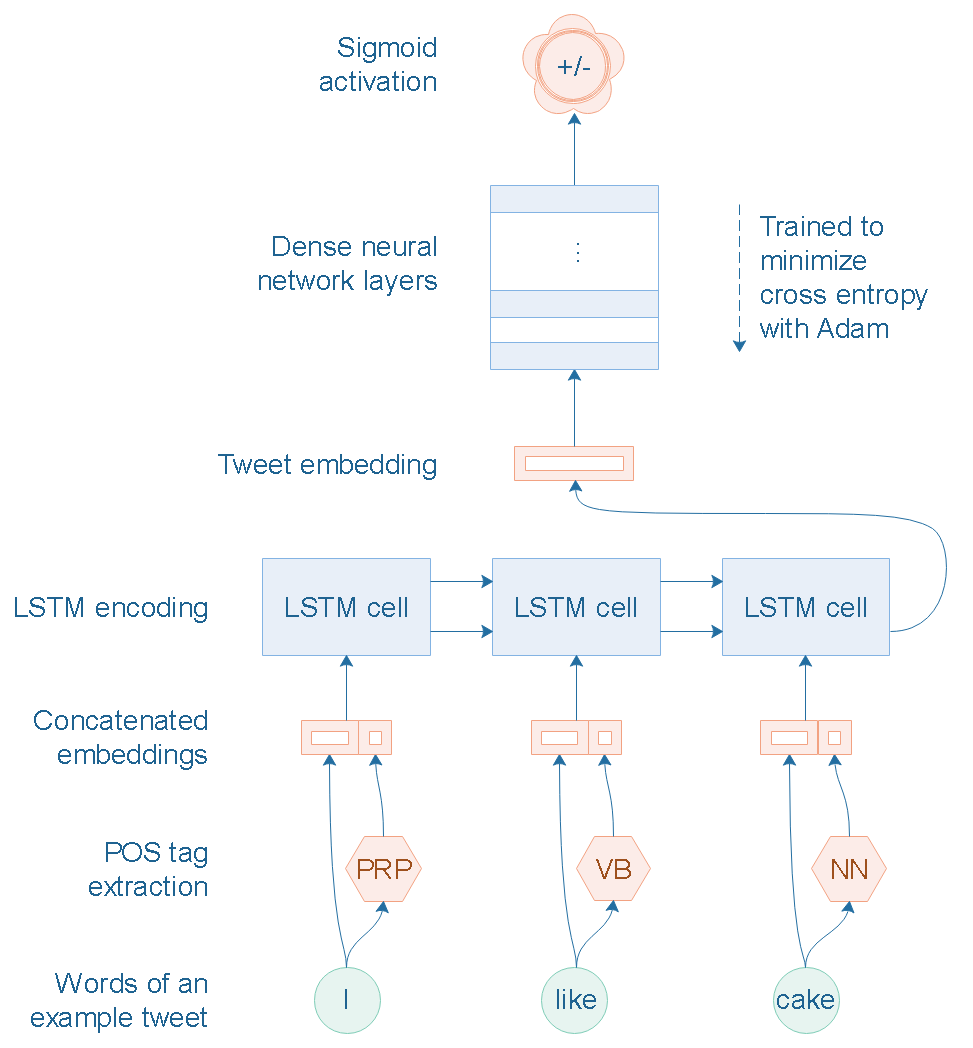
\includegraphics[scale=0.7]{fig/cil_model_pos}
		\caption{The architecture of the POS LSTM model. Image created using Edraw Max \cite{Edraw}.}
		\label{fig:pos_model}
	\end{figure}\\
\indent \textit{Parameters:} We use NLTK's \cite{NLTK} POS-tagger to tag the data. To embed the POS tags we use randomly initialized embeddings of size 50. The available POS tags are described by the Penn Treebank \cite{TREEBANK}. As word embeddings we use Stanford's pre-trained \Glove embeddings trained on Twitter data of size 200.\\
\indent For our implementation of the vanilla model and extensions described above, we use Tensorflow \cite{tensorflow}.  We use NLTK \cite{NLTK} to tokenize the data. We use Tensorflow's Adam optimizer to minimize for cross-entropy for all models. The learning rate for all models is 0.001. During training we use dropout with a rate of 0.5.
	\section{Experiments and results}
	\label{sec:results}
	In this section we present results of different experimental setups.
	\subsection{Baselines}
	In the following we present the results of the baselines described in section \ref{sec:models}. In order to have a consistent and fair comparison of the baselines we use the same seed, we use the same split of 90\% of the full training set as training data and 10\% of the full training data as validation data. We show the test accuracy of the baselines we have tested using the test set, the results are available on Kaggle. Table \ref{tab:baselines} shows a summary of the results.
\begin{table}[h!]
	\centering
        \caption{A summary of the baseline accuracies.}
        \label{tab:baselines}
		\begin{tabular}{|c|c|c|}
			\hline
			Baseline & Validation accuracy & Test accuracy\\
			\hline
			Naive Bayes & 73.4 & 71.7\\
            Average embedding & 75.3 & 69.2\\
			Sentence embedding, architecture 1 & 82.2 & 79.9\\
			Sentence embedding, architecture 2 & 81.7 & 79.6\\
			\hline
		\end{tabular}
\end{table}
	
	\subsection{Model and improvements}
	Here we present the results of experimental setups of our vanilla model and the improvements suggested in section \ref{sec:models}. We use the same seed for each experiment, we use the same split of 90\% of the full training set as training data and 10\% of the full training data as validation data. The results shown are results of the best achieved validation loss for each model respectively. As a result not all models have trained for an equal amount of epochs. Figure \ref{tab:models} shows the results for the vanilla model and improvements \textbf{Important: Read the note at the end of the paper in section \ref{sec:note}.}.
	\begin{table}[h!]
        \caption{Summary of the vanilla model and improvements.}
        \label{tab:models}
		\begin{tabular}{|c|l|c|c|}
			\hline
			Model & embedding & Val. accuracy & Test accuracy\\
			\hline
			Vanilla & Twitter \Glove 25 dim & 86.3 & 85.4\\
			Vanilla & Twitter \Glove 50 dim & 87.2 & 86.2\\
			Vanilla & Twitter \Glove 100 dim & 87.6 & 87.0\\
			Vanilla & Twitter \Glove 200 dim & 88.0 & 87.0\\
			Vanilla & PCA 25 components & 85.6 & NA \\
            POS-model & Twitter \Glove 200 dim & 88.1 & 86.6 \\
			\hline
		\end{tabular} 
	\end{table}
For a closer comparison of the vanilla model and the POS model we trained the models and calculate the validation accuracy and loss in intervals while training. Concretely we calculate validation accuracy and loss 10 times per epoch and train for 20 epochs each. Both models use Stanfords \Glove embeddings trained on twitter data of size 200. The results can be seen in figure \ref{fig:val_comp}.
\begin{figure}
\centering
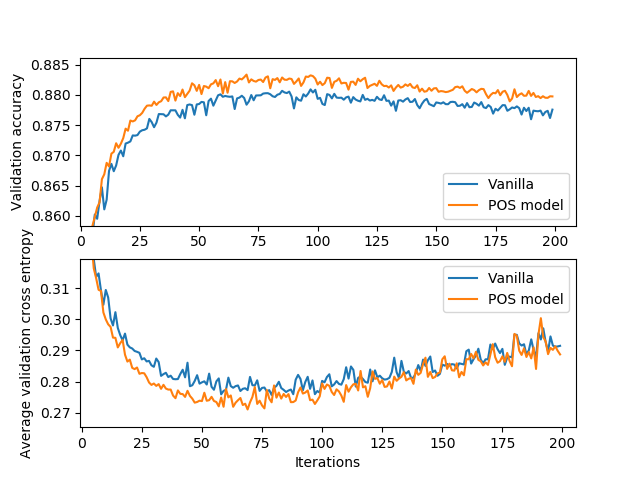
\includegraphics[scale=0.6]{fig/Acc_pos_vs_vanilla.png}
\caption{Comparison of vanilla model and POS model on validation accuracy and loss.}
\label{fig:val_comp}
\end{figure}
    
\section{Discussion}
\label{sec:discussion}
From table \ref{tab:baselines} we can see that the simple naive Bayes baseline managed to obtain a validation and test accuracy in the 70\%. For such a simple model this baseline performed very decently. However, naive Bayes is not able to capture the structure of tweets. A positive tweet with a negation such as \textit{don't worry, I don't hate cake!} can easily be interpreted as negatively sentimented since \textit{worry} and \textit{hate} are more likely to have a higher probability of occurring in a negatively sentimented tweet than positive. A similar performance is obtained by the second baseline, again scoring in the 70\% range. This baseline again does not take into account the structure of the tweet in any way. Additionally this baseline is more prone to overfitting as can be seen by the test accuracy. From the same table however we see the sentence embedding baseline obtained an even higher validation accuracy. Both architectures managed to score in the 80\% which is substantial for a baseline. The Google sentence embeddings in this case are somewhat more able to capture tweet structure than the naive Bayes baseline. However this model suffers tremendously from memory and computational related issues.\\
\indent From table \ref{tab:models} we can clearly see the positive effect of embedding size on the validation accuracy. This shows that in some sense the semantic meaning of words are captured more accurately in higher dimensions. However the gain in accuracy seems to scale logarithmically with the increase in dimensions, meaning one has to make a trade-off between embedding dimensions and computational time, model complexity and validation accuracy.\\
\indent We can see in an attempt to de-noise the data using a PCA the word embeddings became worse compared to Stanford's pre-trained Twitter embeddings of size 25. We assume this is the case since, while a dimension of 200 indeed captures more information about words, when applying PCA we keep less information than Stanford's pre-trained embedding of size 25.\\
\indent However we are able to see a slight improvement when using the POS model over the vanilla model. From figure \ref{fig:val_comp} we can see a consistent improvement in validation accuracy of the POS model over the vanilla model. However since the POS model has a higher model complexity it becomes more prone to over-fitting, as can be seen by the validation loss plot in \ref{fig:val_comp}. Here the validation loss of the POS model increases faster than the vanilla model. However considering the consistent improvement in validation accuracy and the lower validation loss, we conclude there is a definite improvement using the POS model over the vanilla model. As a result we conclude there is information in the POS tags of short texts.

\section{Summary}
Sentiment analysis is an important task in natural language understanding. In this paper we attempt to improve a classical LSTM classifier model by improving word embeddings. We do this by including information about the part of speech (POS). We concluded a noticeable increase in validation accuracy and a decrease in validation loss.

\section{Final Note}  
\label{sec:note}
Please note, the validation accuracies of the POS model in table \ref{tab:models} is not the same as the validation accuracy of the model with chich we made the Kaggle predictions. This is because we failed to notice we commented out where we set the random seed. As a consequence we are not able to reproduce the validation accuracy and the test accuracy by the same model. Instead we have trained 2 separate models.
	\bibliographystyle{ieeetr}
	\bibliography{bib/references.bib}

    \clearpage
    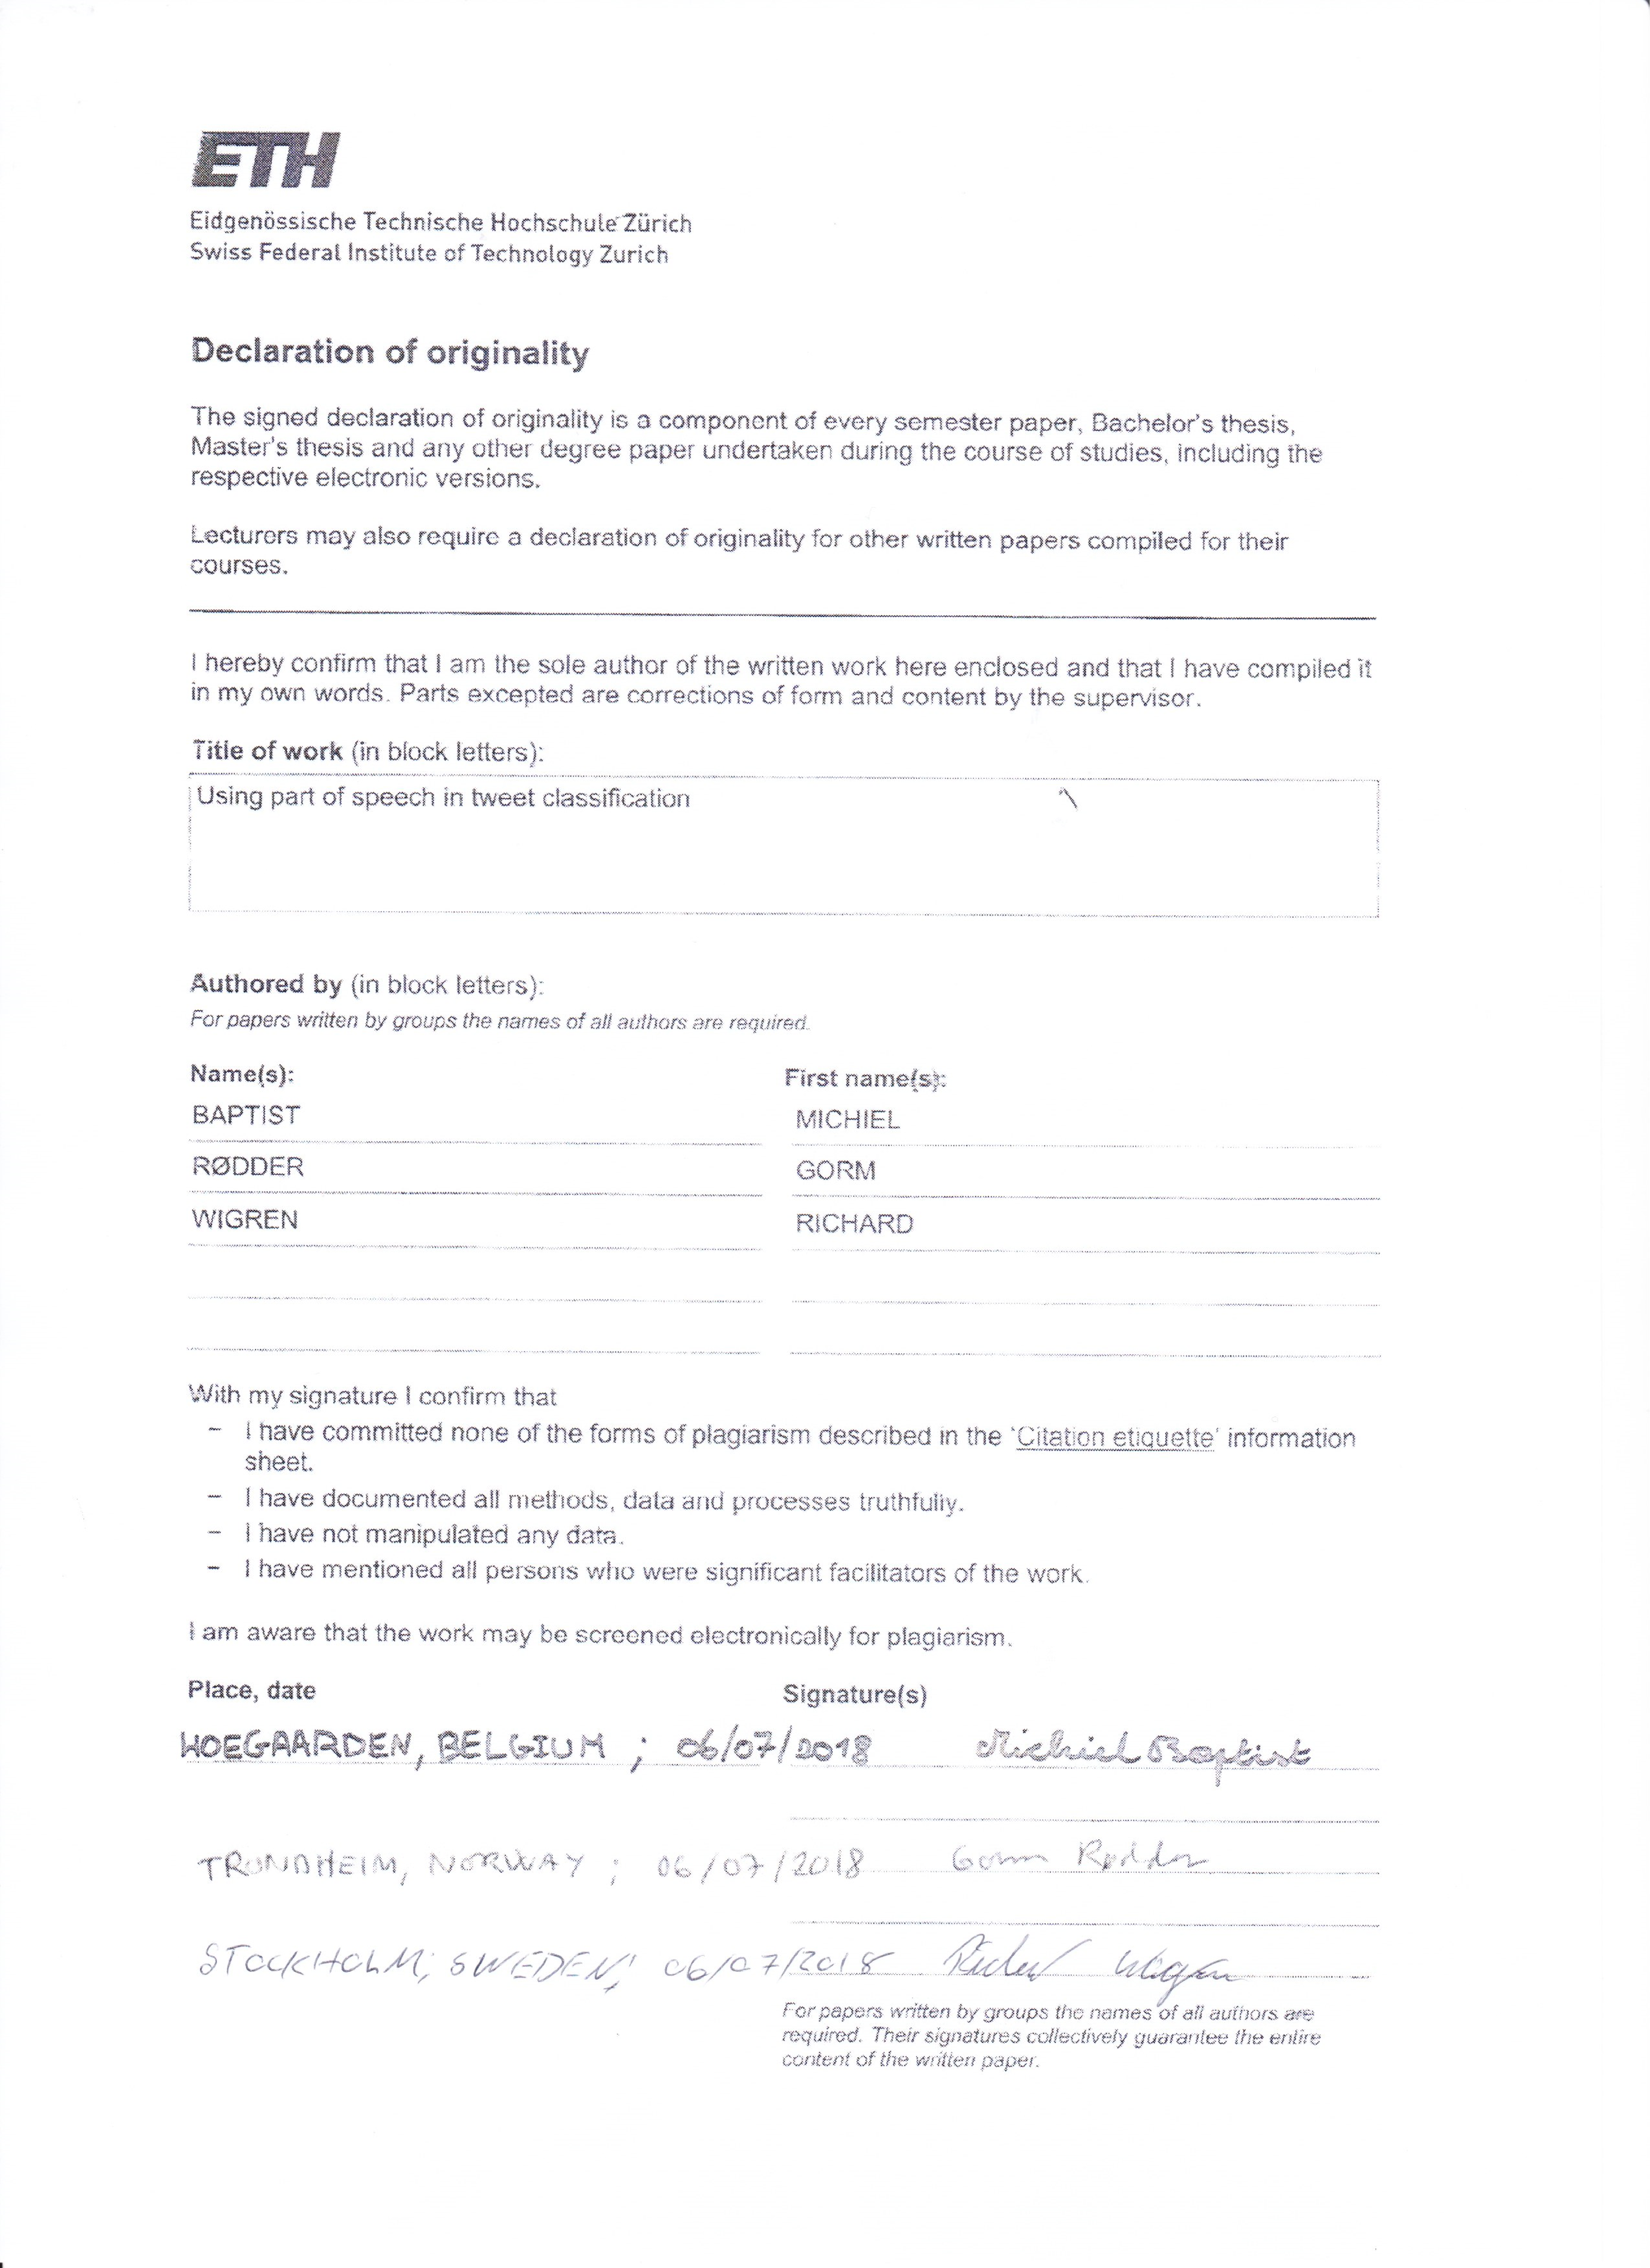
\includepdf{fig/plagerism.pdf}
\end{document}